\documentclass[conference]{IEEEtran}
\IEEEoverridecommandlockouts
\usepackage{cite}
\usepackage{amsmath,amssymb}
\usepackage{graphicx}
\usepackage{booktabs}
\usepackage{url}
\usepackage{textcomp}
\usepackage{xcolor}
% generated by scripts/gen_report_numbers.py - do not edit
\newcommand{\nDirTests}{47}
\newcommand{\nDirTestsFailed}{0}
\newcommand{\nDirChecks}{313}
\newcommand{\nDirChecksFailed}{0}
\newcommand{\nFixedLats}{22}
\newcommand{\nVarLats}{5}
\newcommand{\nRefRuns}{357}
\newcommand{\nRefPassed}{357}
\newcommand{\nRefFailed}{0}
\newcommand{\nRefTxns}{714666}
\newcommand{\nMutants}{28}
\newcommand{\nMutDetPhaseOne}{22}
\newcommand{\nMutDetPhaseTwo}{28}
\newcommand{\nPhaseOneChecks}{122}
\newcommand{\nCovStates}{10}
\newcommand{\nCovTrans}{17}
\newcommand{\nCovReadHit}{50514}
\newcommand{\nCovReadMiss}{18392}
\newcommand{\nCovWriteHit}{49229}
\newcommand{\nCovWriteMiss}{16721}
\newcommand{\nCovConflict}{34752}
\newcommand{\nCovCold}{361}
\newcommand{\nIceFFCtl}{69}
\newcommand{\nIceLutCtl}{42}
\newcommand{\nIceFFMem}{688}
\newcommand{\nIceLutMem}{736}
\newcommand{\nIceFFTot}{757}
\newcommand{\nIceLutTot}{778}
\newcommand{\nPerfRows}{309}
\newcommand{\nHRUni}{0.001}
\newcommand{\nLatUni}{10.50}
\newcommand{\nAmatReadUni}{8.99}
\newcommand{\nHRHot}{0.379}
\newcommand{\nLatHot}{8.46}
\newcommand{\nAmatReadHot}{6.72}
\newcommand{\nHRCon}{0.163}
\newcommand{\nLatCon}{9.49}
\newcommand{\nAmatReadCon}{8.03}
\newcommand{\nHRSeq}{0.589}
\newcommand{\nLatSeq}{6.47}
\newcommand{\nAmatReadSeq}{5.46}
\newcommand{\nHRWri}{0.245}
\newcommand{\nLatWri}{11.54}
\newcommand{\nAmatReadWri}{7.50}
\newcommand{\nHRMix}{0.022}
\newcommand{\nLatMix}{10.62}
\newcommand{\nAmatReadMix}{8.87}
\newcommand{\nHRCor}{0.298}
\newcommand{\nLatCor}{9.23}
\newcommand{\nAmatReadCor}{7.22}
\newcommand{\nHRTag}{0.045}
\newcommand{\nLatTag}{10.25}
\newcommand{\nAmatReadTag}{8.73}
\newcommand{\nLatWriHeavySixteen}{30.24}
\newcommand{\nLatHotSixteen}{20.06}

\newcommand{\todo}[1]{\textcolor{red}{[TODO: #1]}}
\DeclareRobustCommand{\code}[1]{\begingroup\renewcommand{\_}{\char`\_\allowbreak}\texttt{#1}\endgroup}
\def\BibTeX{{\rm B\kern-.05em{\sc i\kern-.025em b}\kern-.08em T\kern-.1667em\lower.7ex\hbox{E}\kern-.125em X}}

\begin{document}

\title{Design and Implementation of a Direct Mapped Cache Controller Using Verilog HDL}

\author{
\IEEEauthorblockN{Ansh}
\IEEEauthorblockA{2401010077\\ B.Tech CSE\\ Newton School of Technology}
\and
\IEEEauthorblockN{Gauri Mehrotra}
\IEEEauthorblockA{2401010170\\ B.Tech CSE\\ Newton School of Technology}
\and
\IEEEauthorblockN{Agnik Misra}
\IEEEauthorblockA{2401010044\\ B.Tech CSE\\ Newton School of Technology}
\and
\IEEEauthorblockN{Lokendra Singh}
\IEEEauthorblockA{2401010254\\ B.Tech CSE\\ Newton School of Technology}
\and
\IEEEauthorblockN{Kartikey Gupta}
\IEEEauthorblockA{2401010214\\ B.Tech CSE\\ Newton School of Technology}
}

\maketitle

\begin{abstract}
This paper presents the design, implementation and verification of a direct-mapped cache controller written in Verilog-2001. The cache has 16 lines of 4 bytes (64~B) in front of a 64~KiB byte-addressable memory, uses a 10/4/2-bit tag/index/offset split, a write-through policy with write allocation, and is controlled by a 10-state finite-state machine. The design is verified purely in simulation (Icarus Verilog): \nDirTests{} directed and edge-case tests, a protocol monitor that checks every transaction, an independent Python reference model compared on \nRefTxns{} randomized and vector transactions, and a mutation study in which \nMutDetPhaseTwo{} of \nMutants{} injected RTL faults are detected. Measured transaction latencies follow closed-form expressions in the main-memory latency $L$ (3, $5{+}L$, $4{+}L$ and $6{+}2L$ cycles for read hit, read miss, write hit and write miss) at every one of \nFixedLats{} tested values of $L$. A technology-mapping estimate (not an implementation) gives \nIceFFTot{} flip-flops and \nIceLutTot{} four-input LUTs for the synthesizable part. No FPGA or silicon timing is claimed.
\end{abstract}

\begin{IEEEkeywords}
cache memory, direct-mapped cache, cache controller, finite-state machine, Verilog HDL, write-through, write-allocate, simulation-based verification, reference model
\end{IEEEkeywords}

%=====================================================================
\section{Introduction}
Processors execute far faster than main memory can supply data, so a small, fast cache holds recently used blocks and exploits temporal and spatial locality~\cite{smith1982,hennessy2017}. Among cache organisations, the direct-mapped cache places each memory block in exactly one line, which makes lookup a single tag comparison and keeps the hit path short~\cite{hill1988}. The price is conflict misses when several active blocks share a line~\cite{hennessy2017}.

This work designs a complete direct-mapped cache \emph{controller}: not only the arrays but also the finite-state machine (FSM) that sequences tag comparison, block refill, write-through and the handshakes with the processor and memory. The emphasis is on a correct, reproducible and explainable design. Every claim in this paper is tied to a saved simulation log in the project repository, and the paper distinguishes carefully between what is \emph{implemented}, \emph{simulated}, \emph{synthesized by a tool}, and merely \emph{proposed}.

\section{Literature Review}
Smith's survey~\cite{smith1982} systematised the design space of cache memories: block size, mapping, replacement and write policies, and their effect on miss ratio. Hill~\cite{hill1988} argued that growing cache sizes and faster hit times make direct-mapped caches increasingly attractive. Jouppi~\cite{jouppi1990} showed that small fully-associative victim and miss caches added to a direct-mapped cache remove many of its conflict misses, which motivates the extension discussed in Section~\ref{sec:future}. The textbook treatment of average memory access time (AMAT), write-through versus write-back and write-allocate versus no-write-allocate is given in~\cite{hennessy2017}.

On the tooling side, the design is written in Verilog-2001~\cite{ieee1364}, simulated with Icarus Verilog~\cite{iverilog}, linted with Verilator~\cite{verilator}, analysed with the Yosys synthesis suite~\cite{wolf2013,yosys}, and its waveforms are inspected with the Surfer viewer~\cite{surfer}. This project contributes a small, fully documented and heavily verified reference implementation rather than a new cache architecture.

\section{Problem Statement}
Design, implement and verify a direct-mapped cache controller for a 16-bit byte-addressable address space with a 64-byte cache and 4-byte blocks that (i) returns correct data for reads and writes, (ii) never returns stale data or responds before the memory has finished, (iii) never performs a duplicate memory write while waiting, (iv) preserves unwritten bytes of a block, and (v) has a precisely documented handshake and timing behaviour that is demonstrably equal to what the implementation does.

\section{Objectives}
\begin{enumerate}
\item Specify and implement a modular Verilog-2001 cache (array, controller, main-memory model, top level).
\item Implement write-through with write allocation and conflict replacement.
\item Verify with directed tests, an always-on protocol monitor, an independent reference model and randomized tests with fixed seeds.
\item Measure hit/miss ratios, latencies and AMAT from actual simulation runs.
\item Check synthesizability and lint cleanliness, and document limitations honestly.
\end{enumerate}

\section{Proposed Solution}
The solution (Fig.~\ref{fig:block}) consists of four Verilog modules: \code{cache\_memory} (arrays and byte merge), \code{cache\_controller} (FSM and datapath registers), \code{main\_memory} (a behavioural, simulation-only 64~KiB model with configurable latency) and \code{cache\_top} (integration and debug ports). The controller latches each CPU request on acceptance, compares the tag and valid bit, and on a miss fetches the aligned 4-byte block and refills the line. After a refill the request is \emph{replayed as a hit}, so read data always comes from the cache array and a write-allocate store reuses the write-hit path. Writes update the cache byte and are written through, byte-wise, to memory before the CPU is answered.

Table~\ref{tab:spec} lists the implemented specification.

\begin{table}[t]
\caption{Implemented specification}\label{tab:spec}
\centering\small
\begin{tabular}{@{}lp{5.2cm}@{}}
\toprule
Parameter & Value \\
\midrule
Address / space & 16-bit byte address, 64~KiB \\
Cache & 16 lines $\times$ 4~B = 64~B, direct mapped \\
Tag / index / offset & $[15{:}6]$ 10 b / $[5{:}2]$ 4 b / $[1{:}0]$ 2 b \\
Per-line storage & 1 valid + 10 tag + 32 data = 43 bits \\
Total logical storage & 688 bits (512 data, 160 tag, 16 valid) \\
Write policy & write-through, write-allocate \\
Replacement & overwrite the selected line on a conflict miss \\
Controller & 10-state Moore-output FSM \\
Reset & synchronous, active high \\
\bottomrule
\end{tabular}
\end{table}

\begin{figure*}[t]
\centering
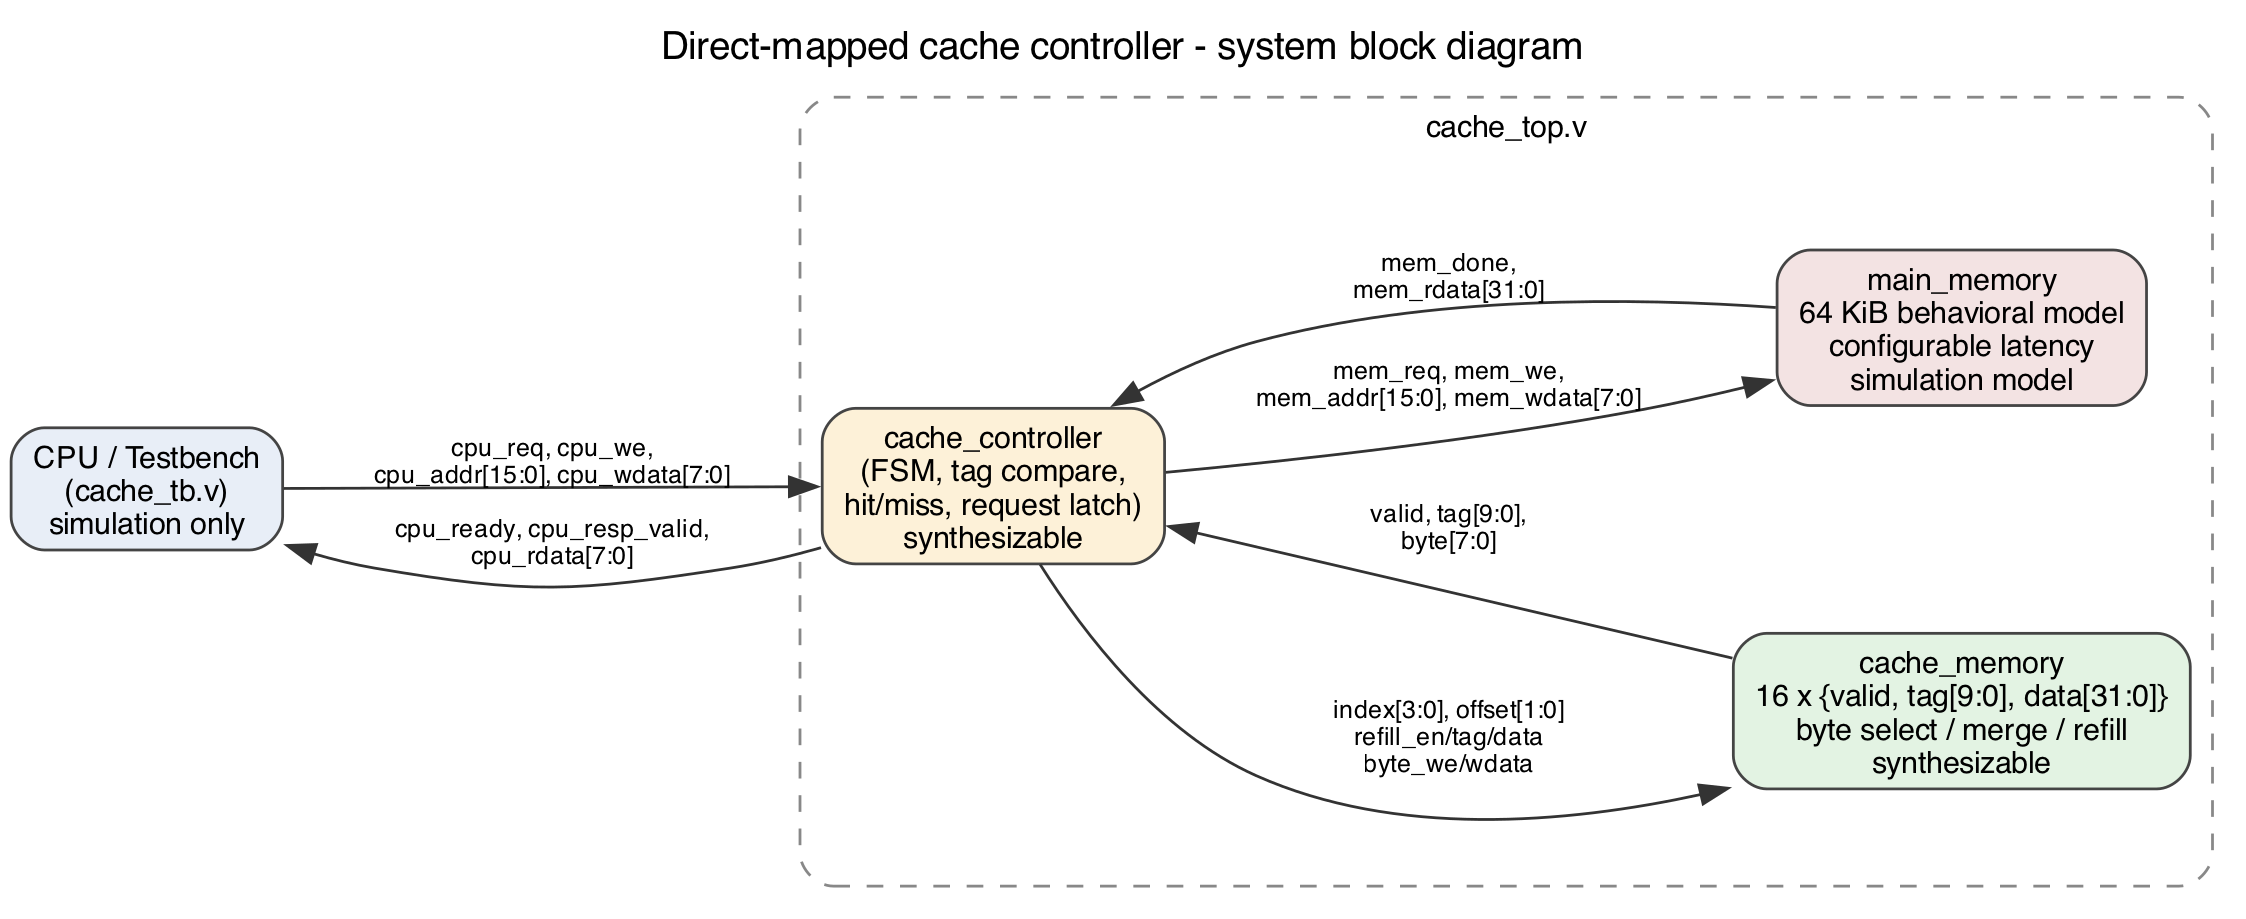
\includegraphics[width=0.85\textwidth]{../diagrams/block_diagram.png}
\caption{System block diagram. The CPU/testbench is simulation-only; \code{cache\_controller} and \code{cache\_memory} are synthesizable; \code{main\_memory} is a behavioural simulation model.}\label{fig:block}
\end{figure*}

\section{System Architecture}
\subsection{Interfaces and handshakes}
\textbf{CPU side.} A request is accepted on a rising clock edge where \code{cpu\_req} and \code{cpu\_ready} are both high; address, write enable and write data are latched at that edge. \code{cpu\_ready} is high only in \code{IDLE}. \code{cpu\_resp\_valid} is high for exactly one cycle in \code{RESPONSE}; \code{cpu\_rdata} is cleared on acceptance and loaded only from the cache array, so it cannot show data from a previous transaction. If \code{cpu\_req} is held high the next request is accepted in the first idle cycle after each response.

\textbf{Memory side.} A single request/\code{done} handshake carries either a block read (aligned address, 32-bit result) or a byte write. The master holds \code{mem\_req}, \code{mem\_we}, address and data stable until the one-cycle \code{mem\_done}. The memory commits a write exactly once, on entering its \code{DONE} state, and ignores requests while busy, so a request still held during the \code{done} cycle cannot be re-accepted.

\textbf{Byte order.} Blocks are little-endian: offset 0 is bits $[7{:}0]$ of the 32-bit block.

\subsection{Timing}
Let $L\ge 1$ be the memory latency in cycles from the first cycle of \code{mem\_req} to the cycle of \code{mem\_done}. The design satisfies, for a transaction measured from the acceptance edge to the edge that samples \code{cpu\_resp\_valid},
\begin{equation}
\begin{split}
T_{\text{rd,hit}}&=3,\qquad T_{\text{rd,miss}}=5{+}L,\\
T_{\text{wr,hit}}&=4{+}L,\quad T_{\text{wr,miss}}=6{+}2L.
\end{split}
\label{eq:lat}
\end{equation}
These expressions were derived from the FSM and then checked, using the measured memory latency, on every transaction of every simulation.

\section{Address Mapping Methodology}
For a 16-bit byte address $a$ with block size $B=4$ and $N=16$ lines,
\begin{equation}
\begin{split}
\text{index}&=\left\lfloor a/B\right\rfloor \bmod N=a[5{:}2],\\
\text{tag}&=a[15{:}6],\quad \text{offset}=a[1{:}0].
\end{split}
\end{equation}
The widths follow from $\log_2 4=2$, $\log_2 16=4$ and $16-4-2=10$. The 16-bit space holds $2^{14}=16384$ blocks, so each line is shared by 1024 blocks, which is why 10 tag bits are needed. A line hits if and only if its valid bit is set and its stored tag equals the address tag; after reset all valid bits are 0, so every first access to a line is a cold miss even though the stored tag resets to 0. The aligned block base is $a\,\&\,\text{0xFFFC}$.

\section{Cache Controller FSM}
The controller (Fig.~\ref{fig:fsm}) has ten states: \code{IDLE}, \code{COMPARE\_TAG}, \code{READ\_HIT}, \code{READ\_MISS}, \code{MEMORY\_READ\_WAIT}, \code{REFILL}, \code{WRITE\_HIT}, \code{WRITE\_MISS}, \code{MEMORY\_WRITE\_WAIT} and \code{RESPONSE}. It is coded as a state register, a combinational next-state block with a \code{default} branch, and non-blocking datapath registers; outputs are Moore.

\begin{figure}[t]
\centering
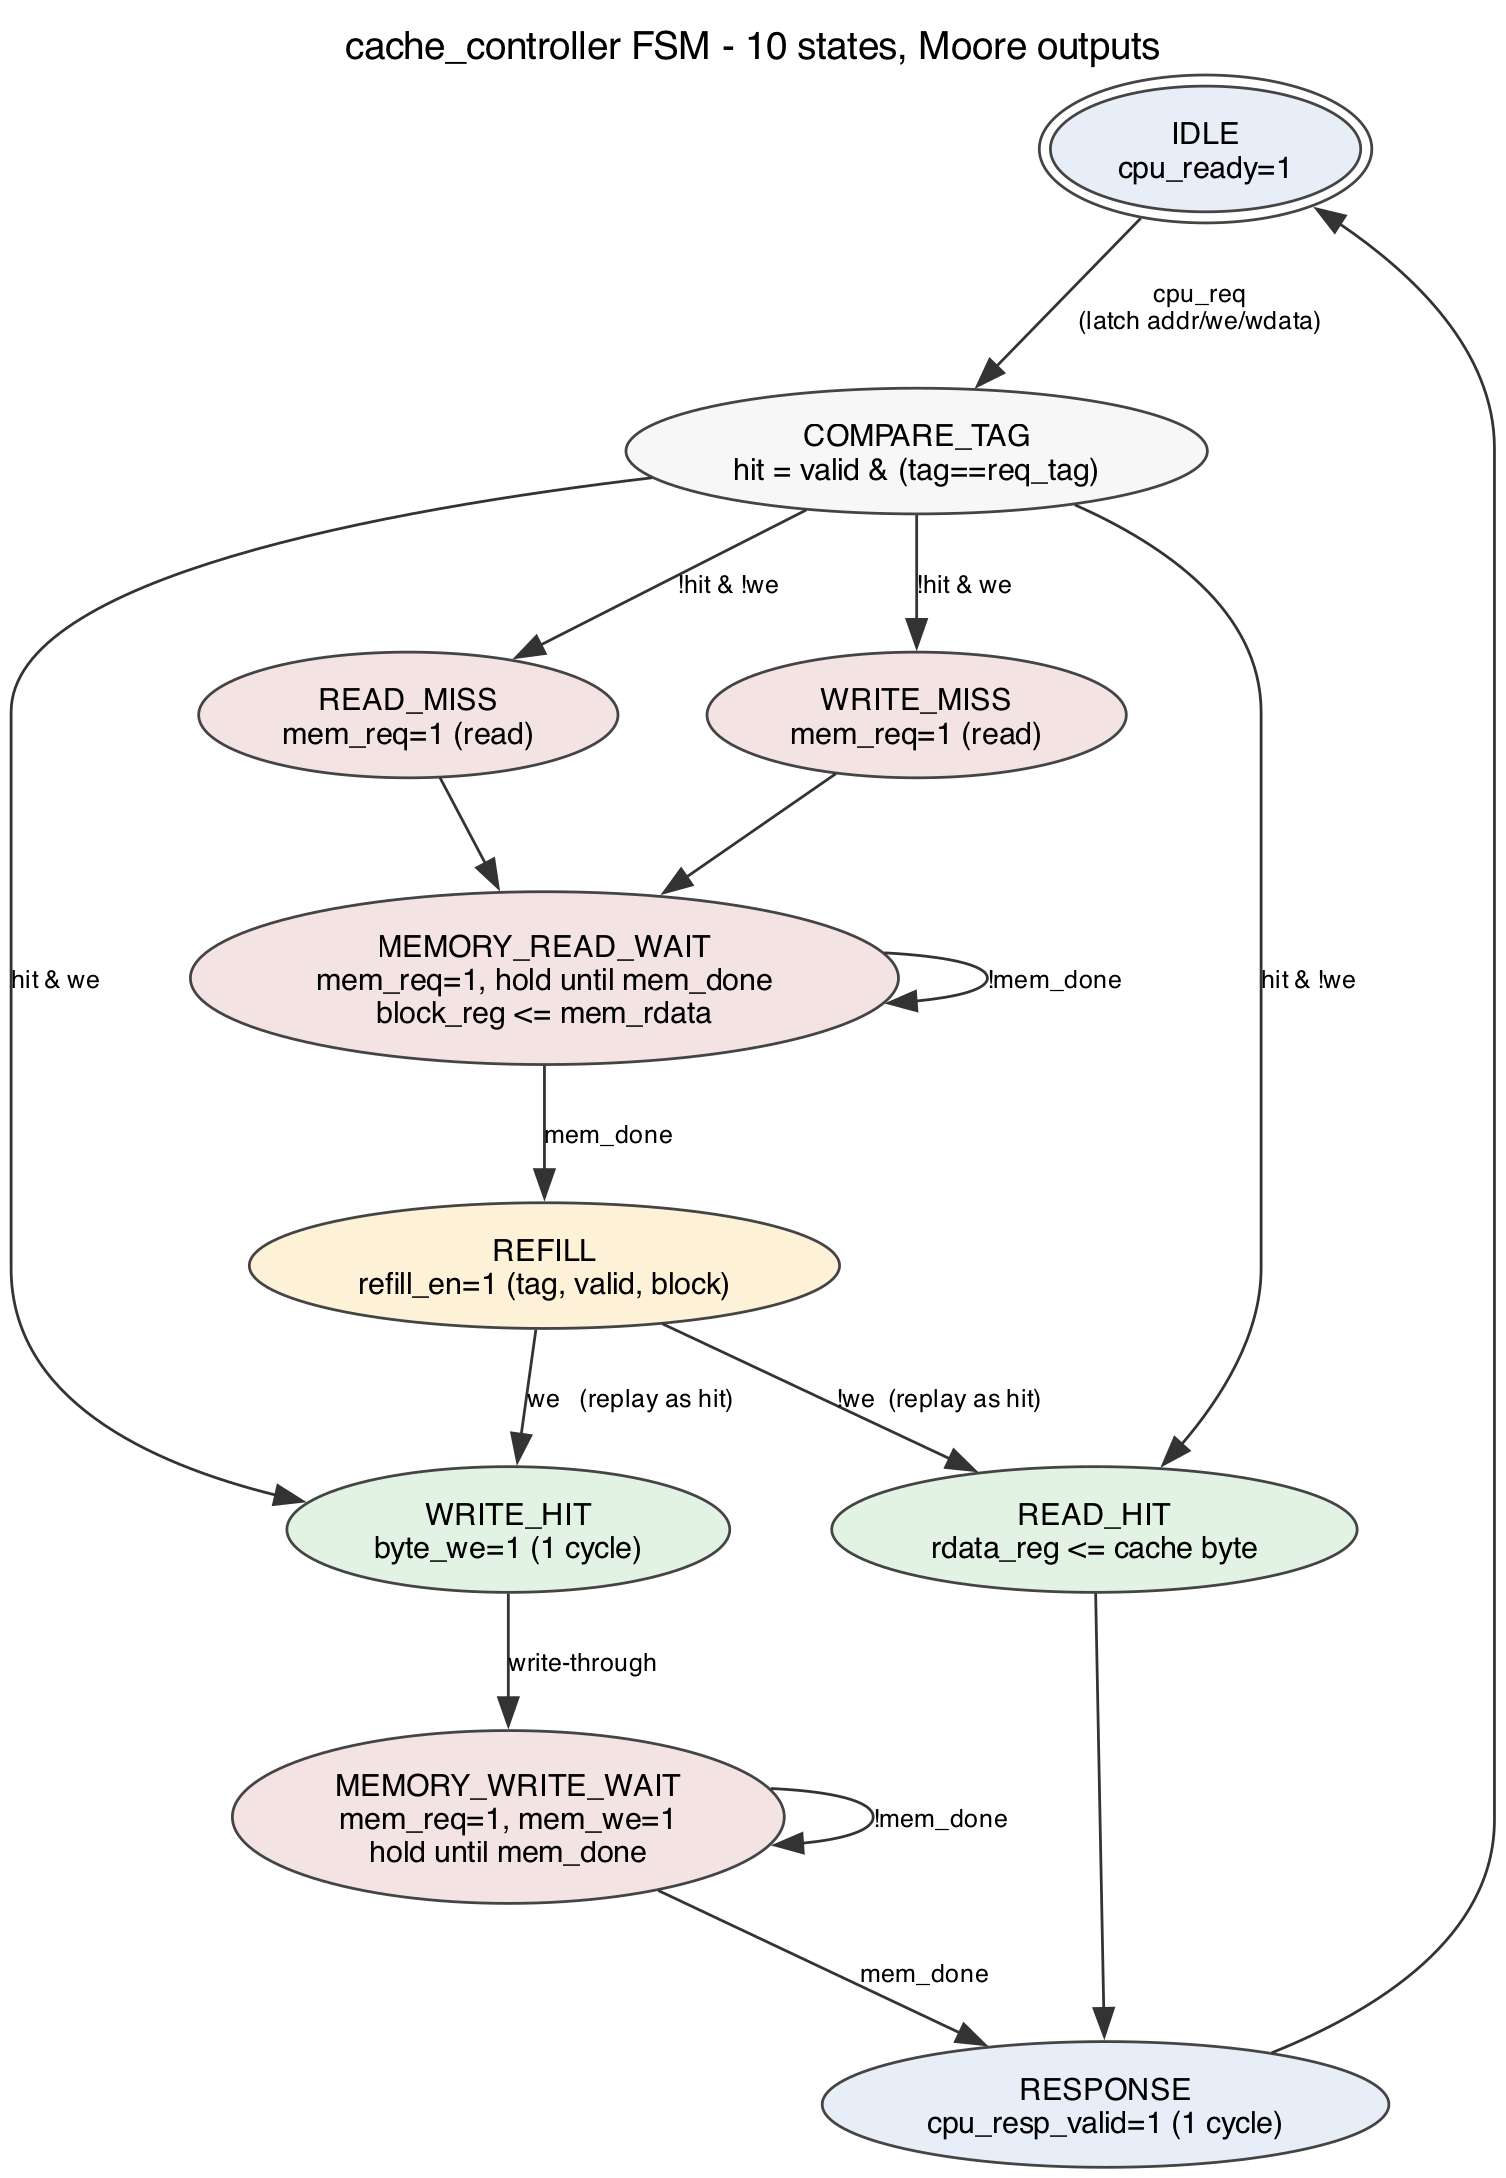
\includegraphics[width=0.92\columnwidth]{../diagrams/fsm_diagram.png}
\caption{Controller FSM. After \code{REFILL} the request re-enters as a hit.}\label{fig:fsm}
\end{figure}

The four transaction paths are:
\begin{itemize}\setlength\itemsep{0pt}
\item read hit: \code{IDLE}, \code{COMPARE\_TAG}, \code{READ\_HIT}, \code{RESPONSE};
\item read miss: \code{COMPARE\_TAG}, \code{READ\_MISS}, \code{MEMORY\_READ\_WAIT}, \code{REFILL}, \code{READ\_HIT}, \code{RESPONSE};
\item write hit: \code{COMPARE\_TAG}, \code{WRITE\_HIT}, \code{MEMORY\_WRITE\_WAIT}, \code{RESPONSE};
\item write miss (write allocate): \code{COMPARE\_TAG}, \code{WRITE\_MISS}, \code{MEMORY\_READ\_WAIT}, \code{REFILL}, \code{WRITE\_HIT}, \code{MEMORY\_WRITE\_WAIT}, \code{RESPONSE}.
\end{itemize}
The byte update strobe is asserted for exactly one cycle in \code{WRITE\_HIT}, so a stall cannot cause a duplicate cache update. \code{MEMORY\_READ\_WAIT} lasts $L$ cycles and \code{MEMORY\_WRITE\_WAIT} lasts $L{+}1$ cycles (the request starts one state earlier for reads); this was established while writing the wait-state test and is documented in the repository. The six unused state codes fall through to \code{IDLE}.

\section{RTL Implementation}
All RTL is Verilog-2001 compiled with \code{iverilog -g2001 -Wall}, with no warnings. \code{cache\_memory} stores the arrays in flip-flops with a synchronous reset that clears valid bits and also tag/data, avoiding X values; its read port is combinational and a function merges a byte into a block while preserving the other three. \code{cache\_controller} contains the FSM and registers. \code{main\_memory} is explicitly a simulation model: its \code{initial} block fills the memory with the deterministic pattern $m[a]=(a[7{:}0]\oplus a[15{:}8])+\text{0x5A}$ modulo 256, so that every byte of a block differs and byte-order bugs are visible.

\emph{Synthesizability.} Yosys \texttt{check -assert} reports no problems (no latches, no multiple drivers). A technology-mapping estimate for iCE40 gives \nIceFFCtl{} flip-flops and \nIceLutCtl{} LUT4 for the controller and \nIceFFMem{} flip-flops and \nIceLutMem{} LUT4 for the cache array, i.e., \nIceFFTot{} flip-flops and \nIceLutTot{} LUT4 in total; the flip-flop count equals the specified 688 storage bits plus 69 controller registers. This is a mapper count only: no place-and-route, timing or power analysis was performed, and the memory model is excluded.

\section{Verification Methodology}
Verification is simulation-based and has six layers.

\textbf{(1) Directed tests.} \nDirTests{} self-checking tests (\nDirChecks{} printed checks at $L{=}4$) implement the plan's 30 directed tests, power-on initialisation, eleven edge cases, a latency test and a coverage test. Edge cases include the address extremes 0x0000 and 0xFFFF, each of the ten tag bits flipped independently at several indices (reads and writes), all 1024 tags on one line, invalid entries aliasing tag~0, and an exhaustive write-and-read sweep of all 65{,}536 addresses. Requests held high across many cycles, and reset applied at every cycle offset during a read miss, a write hit and a write miss, are verified explicitly.

\textbf{(2) Protocol monitor.} Always on: response only for an outstanding request and for exactly one cycle; response only after the exact number of memory operations; exactly one memory-array commit per store; latency equal to~\eqref{eq:lat}; \code{cpu\_rdata} zero until the response; stable memory requests; aligned block reads.

\textbf{(3) Independent reference model.} A Python model written from the specification (no FSM, no handshake) predicts hit/miss, returned byte, memory reads/writes, final cache lines and the full memory image. Eight workload profiles (uniform, hot-set, conflict-heavy, sequential, write-heavy, with resets, address corners, tag patterns) with fixed seeds 1--6 are run at fixed latencies $L\in\{1,2,3,4,8,16\}$ and with pseudo-random per-transaction latency: \nRefRuns{} runs, \nRefPassed{} passed, \nRefTxns{} fixed-latency transactions compared.

\textbf{(4) Latency sweep.} The directed suite is repeated at \nFixedLats{} fixed latencies ($L=0$ clamped to 1, 1--16, 32, 64, 100, 255, 1000) and at \nVarLats{} pseudo-random-latency configurations using a testbench-only memory model.

\textbf{(5) Mutation study.} \nMutants{} single-fault mutants of the RTL are generated; the full directed bench detects \nMutDetPhaseTwo{} of \nMutants{}, whereas the earlier, smaller bench detected \nMutDetPhaseOne{}. One mutant (reset not clearing the arrays) is functionally invisible and is caught only by the power-on X-check, which enforces a stated design decision.

\textbf{(6) Waveform inspection and static checks.} Six scenarios were inspected in the Surfer waveform viewer (Fig.~\ref{fig:wave1},~\ref{fig:wave2}); Verilator lint and Yosys checks were run on the synthesizable modules. GTKWave could not be installed in the development environment, so Surfer was used; the screenshots are of Surfer, not GTKWave.

\section{Results and Discussion}
\textbf{Functional results.} All \nDirTests{} directed tests pass with \nDirChecksFailed{} failures at $L{=}4$, at every fixed latency and with random latency; the reference model agrees on every compared transaction, on the final 16-line cache state and on the full memory image. No RTL defect was found by the extended verification; defects found in test code (a check-width error, a wrong wait-length expectation, a duplicate driver in a test model, a harness crash on X values) were corrected and are logged. The functional-coverage monitor recorded \nCovStates{} of 10 FSM states and \nCovTrans{} of 17 legal transitions (16 of 16 reachable at $L{=}1$), no illegal transition, all 16 indices and 4 offsets for reads and writes, and \nCovCold{} cold and \nCovConflict{} conflict misses. No line or branch coverage tool was run, so no such percentage is claimed.

\textbf{Waveforms.} Fig.~\ref{fig:wave1} shows a cold miss: \code{dbg\_lookup} pulses with \code{dbg\_hit}=0 and the line invalid; \code{mem\_req} stays high until \code{mem\_done}; \code{dbg\_refill} writes the line; the response carries 0x5E exactly once. Fig.~\ref{fig:wave2} shows a write miss with allocation: block fetch, refill, one-cycle byte update, held write-through request, then response.

\begin{figure*}[t]
\centering
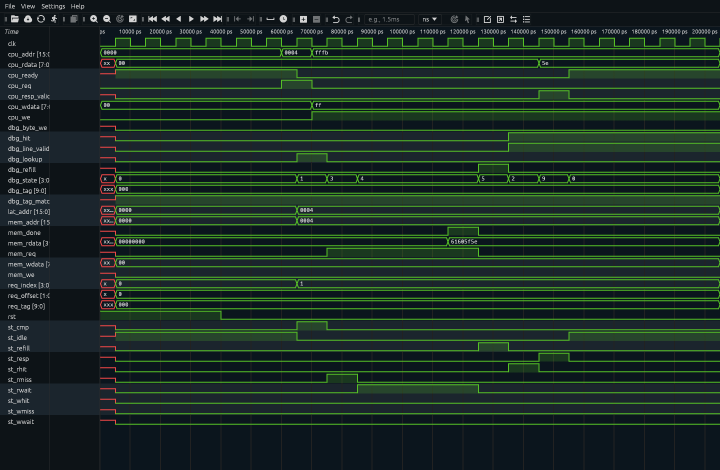
\includegraphics[width=0.8\textwidth]{../results/waveforms/wave_cold_miss_refill.png}
\caption{Cold miss and refill for a read of 0x0004 ($L=4$), rendered by the Surfer viewer from the simulation VCD. State flags: \code{st\_cmp}=\code{COMPARE\_TAG}, \code{st\_rmiss}, \code{st\_rwait}=\code{MEMORY\_READ\_WAIT}, \code{st\_refill}, \code{st\_rhit}, \code{st\_resp}.}\label{fig:wave1}
\end{figure*}

\begin{figure*}[t]
\centering
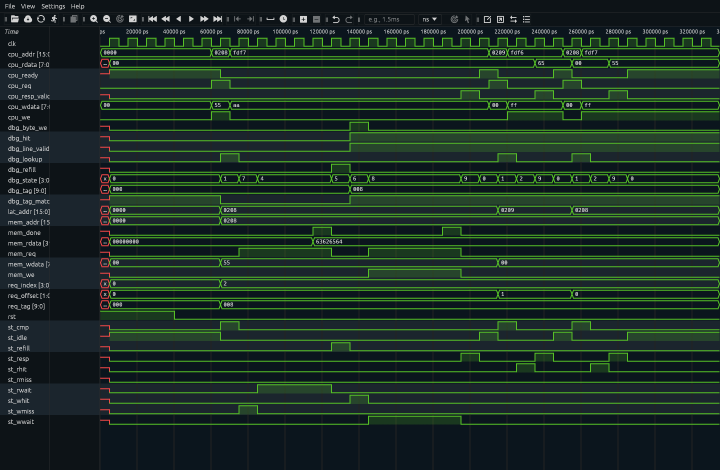
\includegraphics[width=0.8\textwidth]{../results/waveforms/wave_write_miss_alloc.png}
\caption{Write miss with allocation for a write of 0x55 to 0x0208 ($L=4$): \code{st\_wmiss}, read wait, \code{st\_refill}, \code{st\_whit} (one-cycle \code{dbg\_byte\_we}), \code{st\_wwait} with \code{mem\_we} and \code{mem\_wdata}=0x55, \code{st\_resp}.}\label{fig:wave2}
\end{figure*}

\textbf{Latency.} Fig.~\ref{fig:lat} plots the measured transaction latencies against $L$; they coincide with~\eqref{eq:lat} at all tested values. Writes are costly because write-through stalls the CPU for the memory write even on a hit.

\begin{figure}[t]
\centering
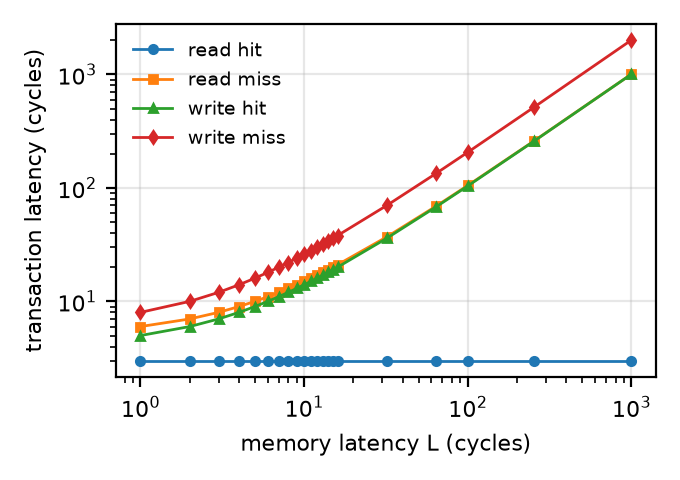
\includegraphics[width=0.95\columnwidth]{../diagrams/fig_latency_vs_L.png}
\caption{Measured transaction latency versus memory latency $L$ (from \code{results/phase2\_latency\_sweep.txt}).}\label{fig:lat}
\end{figure}

\section{Performance Analysis}
\textbf{Definitions.} Hit ratio $=\text{hits}/\text{requests}$, miss ratio $=1-$ hit ratio, and
\begin{equation}
\text{AMAT}=T_\text{hit}+\text{MR}\times T_\text{miss\,penalty}.
\label{eq:amat}
\end{equation}
For reads, $T_\text{hit}=3$ and the penalty is $(5{+}L)-3=2{+}L$ cycles. Because every write pays the write-through latency, eq.~\eqref{eq:amat} applies to reads only; for mixed traffic a class-weighted average of~\eqref{eq:lat} is used, and it equals the measured average latency (it is a consistency check, not independent evidence). All values are simulated clock cycles; no clock frequency or physical timing is assumed.

\textbf{Workloads.} Eight synthetic profiles of 2500 requests with seeds 1--6 were run on the actual RTL; Table~\ref{tab:perf} shows means at $L=4$.

\begin{table}[t]
\caption{Measured performance at $L=4$ (mean over 6 seeds, 2500 requests)}\label{tab:perf}
\centering\small
\begin{tabular}{@{}lrrr@{}}
\toprule
Workload & Hit ratio & Avg. latency & AMAT$_\text{read}$ \\
\midrule
uniform random      & \nHRUni & \nLatUni & \nAmatReadUni \\
hot set             & \nHRHot & \nLatHot & \nAmatReadHot \\
conflict-heavy      & \nHRCon & \nLatCon & \nAmatReadCon \\
sequential          & \nHRSeq & \nLatSeq & \nAmatReadSeq \\
write-heavy         & \nHRWri & \nLatWri & \nAmatReadWri \\
with resets         & \nHRMix & \nLatMix & \nAmatReadMix \\
address corners     & \nHRCor & \nLatCor & \nAmatReadCor \\
tag patterns        & \nHRTag & \nLatTag & \nAmatReadTag \\
\bottomrule
\end{tabular}
\end{table}

The near-zero hit ratio of uniform random traffic is expected: a 64-byte cache covers $0.1\%$ of a 64~KiB space. Sequential traffic achieves the highest hit ratio through spatial locality of the 4-byte block, and hot-set traffic benefits from temporal locality. The conflict profile (three indices, six tags) shows how aliasing defeats a direct-mapped cache. The write-heavy profile has the highest average latency (\nLatWri{} cycles at $L{=}4$; \nLatWriHeavySixteen{} versus \nLatHotSixteen{} for the read-dominated hot-set profile at $L{=}16$), quantifying the cost of write-through without a write buffer. These results describe synthetic workloads only and say nothing about real programs.

\begin{figure}[t]
\centering
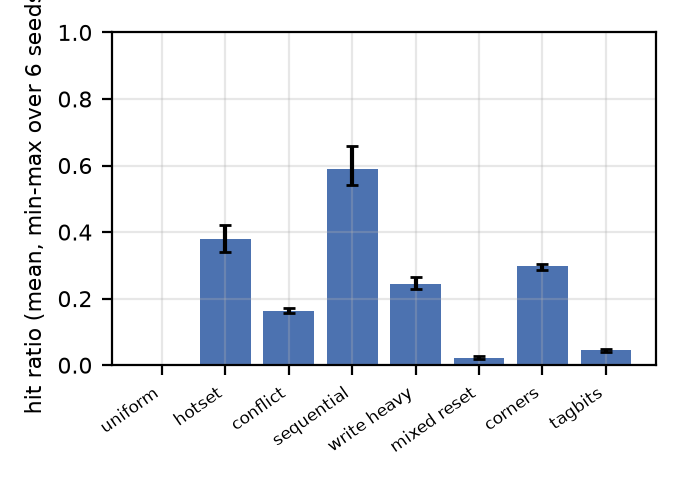
\includegraphics[width=0.95\columnwidth]{../diagrams/fig_hit_ratio.png}
\caption{Hit ratio by workload at $L=4$ (bars: mean, whiskers: min--max over seeds).}\label{fig:hit}
\end{figure}

\section{Individual Contributions}
Table~\ref{tab:contrib} is a template. Names and actual contributions have \emph{not} been supplied and are therefore left as placeholders; no contribution is claimed for any member.

\begin{table}[t]
\caption{Individual contributions (to be completed by the team)}\label{tab:contrib}
\centering\small
\begin{tabular}{@{}lp{5.3cm}@{}}
\toprule
Member & Actual contribution \\
\midrule
1 & \todo{name and contribution} \\
2 & \todo{name and contribution} \\
3 & \todo{name and contribution} \\
4 & \todo{name and contribution} \\
5 & \todo{name and contribution} \\
\bottomrule
\end{tabular}
\end{table}
\todo{disclose AI-assistant use for code, test and documentation generation in the form required by the university; see \code{docs/individual\_contributions.md}}

\section{Limitations}
(i) Verification is simulation-only (Icarus Verilog); there is no formal proof, no gate-level or FPGA/ASIC timing, and the synthesis numbers are mapper estimates. (ii) Only functional coverage was measured; no line/branch/toggle coverage is claimed. (iii) One outstanding request, no pipelining, no write buffer; every write stalls for the memory latency. (iv) Main memory is a behavioural model with a 16-bit latency counter (latencies above 65535 are unsupported); random-latency testing uses a testbench-only memory. (v) Cache arrays are flip-flops with a reset on every entry, which is simple but not area-efficient. (vi) Workloads are synthetic. (vii) The waveform viewer was Surfer rather than GTKWave. (viii) The Python model's latency column restates the documented timing contract; timing itself is verified separately by the monitor.

\section{Future Scope}\label{sec:future}
(a) A small fully-associative victim cache to absorb conflict misses~\cite{jouppi1990}; (b) set-associative mapping with a replacement policy; (c) a write buffer or write-back policy with dirty bits to hide write latency; (d) a pipelined or non-blocking interface; (e) word-wide CPU data; (f) block-RAM storage for the arrays; (g) FPGA place-and-route to obtain real timing and area; (h) formal verification of the handshake properties; (i) line/branch coverage measurement.

\section{Conclusion}
A direct-mapped, write-through, write-allocate cache controller was designed in Verilog-2001 and verified in simulation. All directed tests, edge cases, \nRefTxns{} reference-model comparisons and latency sweeps pass; the measured latencies match closed-form expressions at every tested memory latency; and a mutation study shows the tests detect the injected faults. The documentation, scripts and logs allow the entire evidence to be regenerated with two commands. The work does not claim FPGA or silicon results.

\begin{thebibliography}{00}
\bibitem{smith1982} A. J. Smith, ``Cache memories,'' \emph{ACM Computing Surveys}, vol. 14, no. 3, pp. 473--530, Sep. 1982, doi: 10.1145/356887.356892.
\bibitem{hill1988} M. D. Hill, ``A case for direct-mapped caches,'' \emph{Computer}, vol. 21, no. 12, pp. 25--40, Dec. 1988, doi: 10.1109/2.16187.
\bibitem{jouppi1990} N. P. Jouppi, ``Improving direct-mapped cache performance by the addition of a small fully-associative cache and prefetch buffers,'' in \emph{Proc. 17th Int. Symp. Computer Architecture (ISCA)}, Seattle, WA, USA, May 1990, pp. 364--373.
\bibitem{hennessy2017} J. L. Hennessy and D. A. Patterson, \emph{Computer Architecture: A Quantitative Approach}, 6th ed. Morgan Kaufmann (Elsevier), 2017, ISBN 978-0-12-811905-1.
\bibitem{ieee1364} \emph{IEEE Standard Verilog Hardware Description Language}, IEEE Std 1364-2001, 2001 (superseded by IEEE Std 1364-2005).
\bibitem{wolf2013} C. Wolf and J. Glaser, ``Yosys -- A free Verilog synthesis suite,'' in \emph{Proc. Austrochip Workshop on Microelectronics}, Oct. 2013, pp. 47--52.
\bibitem{iverilog} \emph{Icarus Verilog} (version 13.0 used). [Online]. Available: \url{https://steveicarus.github.io/iverilog/}
\bibitem{yosys} \emph{Yosys Open SYnthesis Suite} (version 0.71 used). [Online]. Available: \url{https://yosyshq.net/yosys/}
\bibitem{verilator} \emph{Verilator} (version 5.054 used). [Online]. Available: \url{https://www.veripool.org/wiki/verilator}
\bibitem{surfer} \emph{Surfer waveform viewer} (version 0.7.0 used). [Online]. Available: \url{https://surfer-project.org/}
\end{thebibliography}

\end{document}
